% !TEX root = ../main.tex

\chapter{Inhaltsspezifische Überschrift}
%\chapter{Very Specific Title}
\label{sect:corechapter}

% Kernstück der Arbeit (eventuell auch in mehrere Kapitel unterteilt). Hier wird konkret vorgestellt, was entwickelt wurde und wie dies von statten ging.
% This chapter (maybe split in multiple) is the main part of the thesis. It presents what was realized, how things were realized, 

As already stated before in chapter , every chapter or section should start with some introducing words.
Due to the fact that this chapter (or potentially multiple chapters) presents the authors efforts, each section and chapter shall provide analogous to its introduction some concluding words, summarizing the findings and achievements of the specific section or chapter.


% Alles aus dem Grundlagen-Kapitel kann ohne weitere Erklärung genutzt werden. nicht zu erwarten ist, dass der leser über nicht präsentierte Zusatzinformationen zum Thema verfügt.
% The information presented before in the background chapter can be used without further explanation. However you should not assume that the reader knows further details on the topic which were not presented in this thesis.
\section{Different Citation Types}

During the writing of a thesis work, ideas and contributions provided by other people then the author have to be declared as such.
This is done using citations.
In general, there are two different types of citations.
The first type of citation is the literal citation.
It is only used if text is copied directly without modification from others.
In this case the citation is surrounded by quotes "".
For instance:
\begin{center}
  Wikipedia states that \enquote{Wörtliche Zitate sollten eingesetzt werden, wenn nicht nur der Inhalt der Aussage, sondern auch deren Formulierung von Bedeutung ist} .
\end{center}
Nonetheless, the author has to make unambiguously clear where the citation originates from.
In case of the wikipedia citation above this is done with:  .


The second citation type is the more frequent used reference using the \textbackslash cite\{\} command presented in Sect.
This citation type is used if no literal citation is used.
For instance:
\begin{center}
  If not only the content of a statement is of importance but also the original wording, then literal citation using quotes has to be used  .
\end{center}
Such references have to follow directly the first statement taken from other sources.

The following example shows how this looks for bigger paragraphs.
The same colored parts refer to the same source.

\begin{flushleft}
  \textcolor[rgb]{1,0,0}{Welche Theorien standardmäßig von einem Programm zur Lösung von SMT-Problemen unterstützt werden hängt vom konkret verwendeten Programm ab .
    Zur Vereinheitlichung der Beschreibung von Theorien, so wie der Eingabe- und Ausgabesprache für Programme die SMT-Probleme lösen wurde der SMT-LIB Standard verfasst.}
  \textcolor[rgb]{0.2,0.8,0.2}{Aktuell befindet sich dieser von der SMT-LIB Initiative formulierte Standard in Version 2.0 .}
  \textcolor[rgb]{0,0.8,1}{Zu diesen Theorien gehören die Theorie der Felder (engl. \textit{arrays}), der Bit-Vektoren fester Größe, der booleschen Operatoren, der Fließkommazahlen, der Ganzzahlen, der reellen Zahlen und der Kombination von reellen und ganzen Zahlen.}
\end{flushleft}

Please ensure that the visual look of the automatically generated bibliography is consistent and the printed information is complete.
For instance:
\begin{itemize}
  \item the separation of words at the end of a line should be adequate
  \item the ISBN, DOI, etc. are formatted the same way for every bibliography entry
  \item every web-sources accessing-date is stated
  \item URLs are displayed the way they are intended to (e.g. underscores in copied links are interpreted by latex as commands and not displayed unless the url is surrounded by \textbackslash url\{\} or backslashes are interpreted as escaping characters and should be replaced with \textbackslash textbackslash)
\end{itemize}
It is the responsibility of the author of a thesis to ensure that all relevant information about the used literature is readable in the printed version of the thesis.

The next section gives advice on figures used in the document and extends the citation concept accordingly.


\section{Citations and Advice on Illustrations}

Similar to textual content, pictures may originate from other publications, too.
Thus, they have to be declared as results of work from others.
In case the figure is not modified in any way this can be done by adding a correspondent citation in the figures caption.
If the figure has been redrawn or modified the reference can be given as shown below:
\begin{figure}[H]
  \centering
  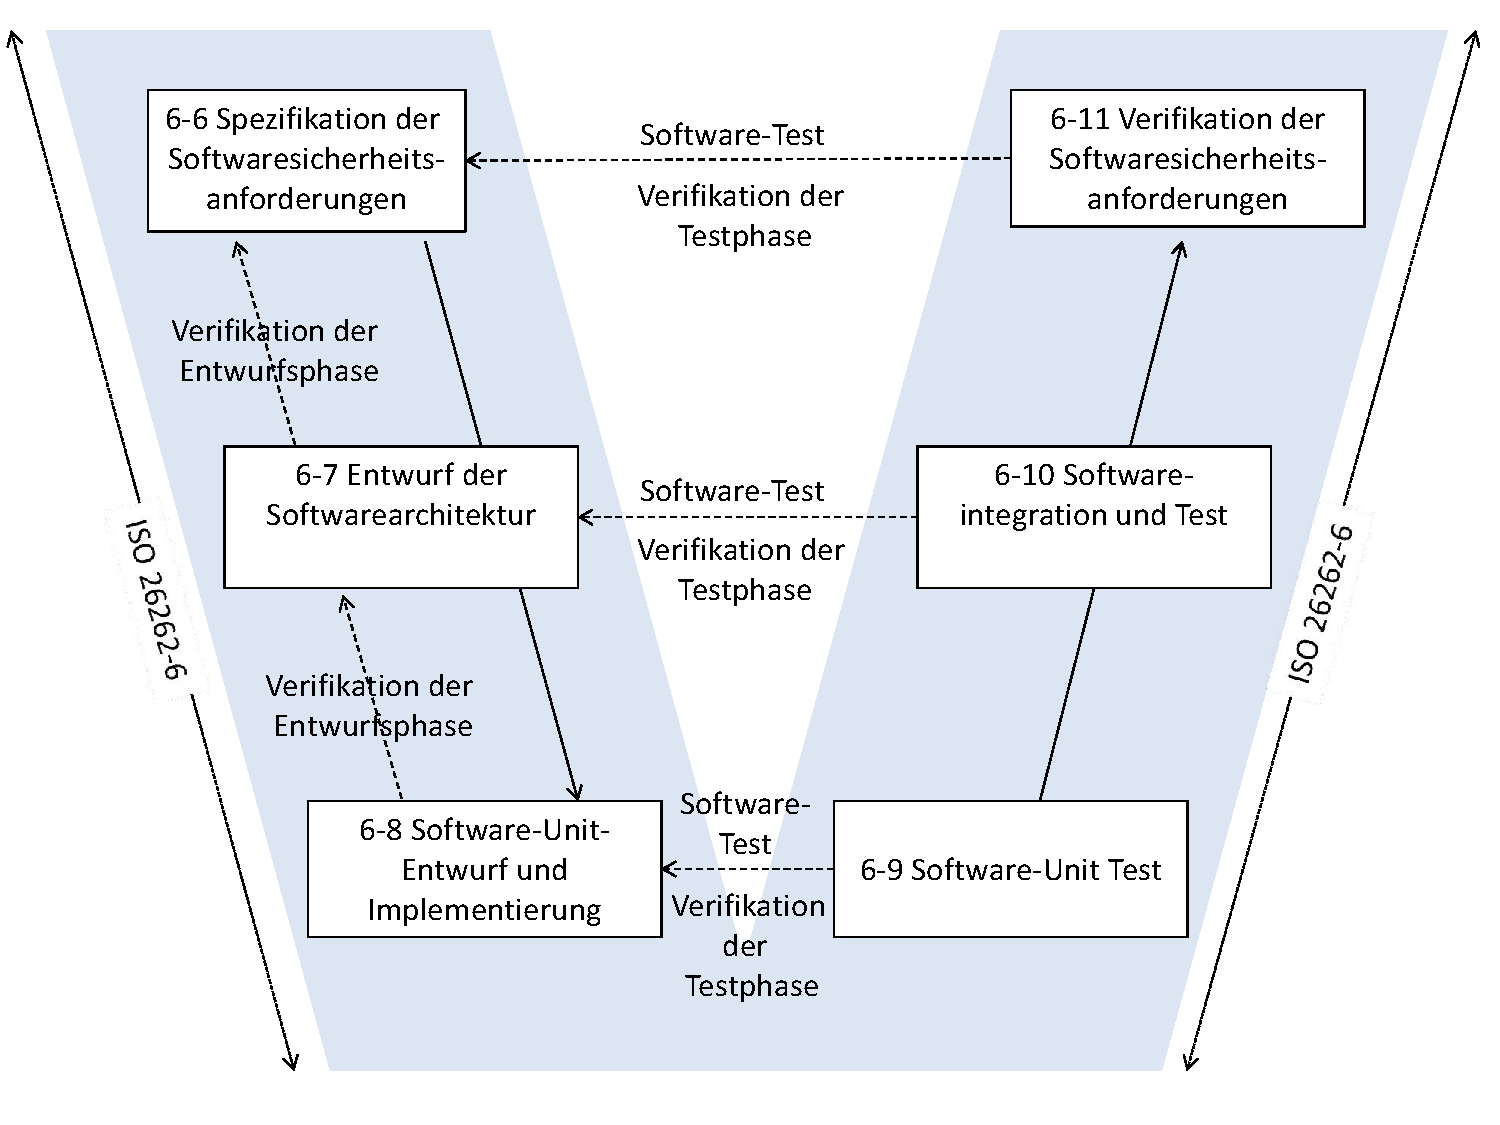
\includegraphics[width=0.80\textwidth]{figures/V-Modell.pdf}
  \caption{V-Modell correspondent to ISO 26262-6 (drawing after)}
  \label{fig:vmodell}
\end{figure}

The author might even differentiate between different figure-citation-types.
Those could be:
\begin{itemize}
  \item taken from \textit{(exact copy of the figure)}
  \item partly taken from \textit{(parts of the figure are taken from the specified source, others were added by the author)}
  \item adaption/extension of
  \item redrawing of \textit{(the figure has been redrawn)}
\end{itemize}
If such descriptions or correspondent abbreviations are used the author should specify upfront the semantic and syntax at the beginning of the thesis.
The important thing here is not which words were used but that it is clear which parts are whose work.
\\\\
\textsl{\textcolor[rgb]{0.75,0.75,0.75}{It follows an example for a bad structuring of paragraphs and transition between such since the quality of figures does not relate to figure citations.}}
Also it is not recommendable to use fonts, \textcolor[rgb]{1,1,0}{colors} and other \textsl{\textit{\colorbox[rgb]{1,1,0.6}{\textcolor[rgb]{0.8,1,0.8}{styling}}}} elements (even in figures) which cannot be read easily.
\\\\
Figures should always be provided as vector graphics, e.g. *.svg or *.pdf files.
The benefit of such formats is their scalability without loss of quality.
Unfortunately, many pictures are not provided as such.
Hence, schemata etc. need often to be redrawn.
Some tools supporting the creation of vector graphics are:
\begin{itemize}
  \item inkscape (open source)
  \item powerpoint (create a slide composed of shapes and store it as *.pdf file) or word/excel\\
        (this should work with open office too)
  \item to be completed ...
\end{itemize}
Please note that importing non vector graphics, e.g. bitmaps, by the mentioned tools will not convert them into vector graphics.
Another aspect which should be addressed regarding figures in latex documents is the size of text inside figures.
Due to scale operations on figures (see \ref{fig:vmodell} where the width of the figure is set to 80 percent of the width of the region where text can be shown) the size of text labels in figures may change.
However, the size of the smallest text on a figure should never be smaller than the smallest text-size of the rest of the document.
Moreover the sizes of texts on figures should not change arbitrary between illustrations.

After this part of many theses follows an evaluation.
Some important points regarding the evaluation part are mentioned in the following chapter.